\documentclass[class=beamer, crop=false]{standalone}

\usepackage{tikz}
\usepackage{subcaption}
\usetikzlibrary{calc}


\begin{document}

% \begin{figure}[0.8\linewidth]
  % \centering
  \begin{columns}[t]
      \centering
      \column{0.4\textwidth}
      \centering
    
      \resizebox{0.5\columnwidth}{!}{%
      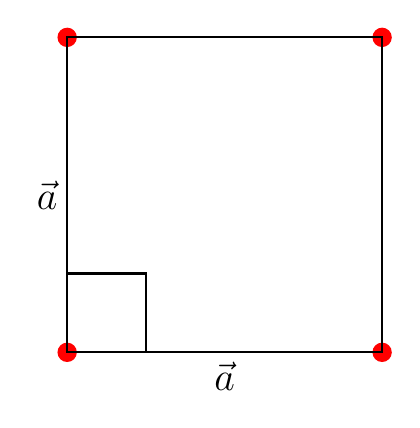
\begin{tikzpicture}
        \def\a{4}  % length of side a
            
        % Calculate the coordinates of the points
        \coordinate (A) at (0, 0);
        \coordinate (B) at (\a, 0);
        \coordinate (C) at (\a, \a);
        \coordinate (D) at (0, \a);
    
        \fill[red]  (A) circle(3.5pt) (B) circle(3.5pt) (C) circle(3.5pt) (D) circle(3.5pt);
            
        % Draw the square unit cell
        \draw[thick] (A) -- (B) -- (C) -- (D) -- cycle;
    
        % Draw right angle
        \draw[thick] (0,1) -- (1,1) -- (1,0);
    
        %Draw lattice parameters
        \node[left] at ($(A)!0.5!(D)$) {\Large $\vec{a}$};
        \node[below] at ($(A)!0.5!(B)$) {\Large $\vec{a}$};
        
      \end{tikzpicture}}
    
      
      \vspace{0.5ex}
    
      {\footnotesize\textbf{(a)} Square Cell}
    
      \column{0.4\textwidth}
        
      \resizebox{0.6\columnwidth}{!}{%
      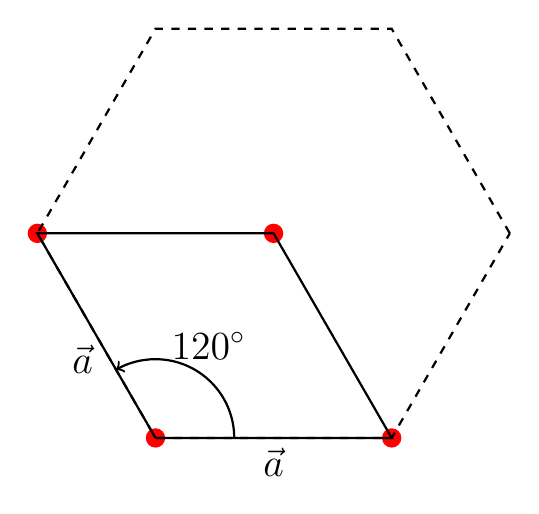
\begin{tikzpicture}
        \def\a{3}  % length of side a
            
        Calculate the coordinates of the points
        \coordinate (A) at (0:\a);
        \coordinate (B) at (60:\a);
        \coordinate (C) at (120:\a);
        \coordinate (D) at (180:\a);
        \coordinate (E) at (240:\a);
        \coordinate (F) at (300:\a);
        \coordinate (G) at (0,0);
       
        % Creates nodes at vertices
        \fill[red]  (D) circle(3.5pt) (E) circle(3.5pt) (F) circle(3.5pt) (G) circle(3.5pt);
        
        % Draw the hexagon boundary
        \draw[thick,dashed] (A) -- (B) -- (C) -- (D) -- (E) -- (F) -- (A);
    
        % Draw the cell
        \draw[thick] (E) -- (F) -- (G) -- (D) -- (E); 
            
        %Draw lattice parameters
        \node[anchor={60}] at ($(D)!0.5!(E)$) {\Large $\vec{a}$};
        \node[below] at ($(E)!0.5!(F)$) {\Large $\vec{a}$};
    
        % Optional: add angle markers
        \draw[thick, ->] (E) ++(1,0) arc[start angle=0, end angle=120, radius=1] node[midway,anchor={-120}] {\Large $120^\circ$};
        
      \end{tikzpicture}}
    
      {\footnotesize\textbf{(b)} Hexagon Cell}
    
    \end{columns}
    \vspace{1em}
    \begin{columns}[t]
      \centering
      \column{0.25\textwidth}
    
      \resizebox{0.9\columnwidth}{!}{%
      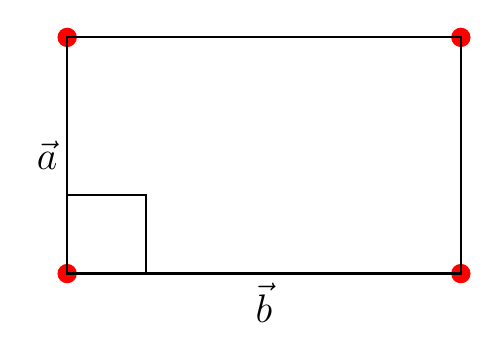
\begin{tikzpicture}
        \def\a{5}  % length of side a
        \def\b{3}  % length of side b
        \def\y{5}
    
        % Calculate the coordinates of the points
        \coordinate (A) at (0, 0);
        \coordinate (B) at (\a, 0);
        \coordinate (C) at (\a, \b);
        \coordinate (D) at (0, \b);
    
        % Creates nodes at vertices
        \fill[red]  (A) circle(3.5pt) (B) circle(3.5pt) (C) circle(3.5pt) (D) circle(3.5pt);
        
        % Draw right angle
        \draw[thick] (0,1) -- (1,1) -- (1,0);
    
        % Draw the rectangular unit cell
        \draw[thick] (A) -- (B) -- (C) -- (D) -- cycle;
       
        %Draw lattice parameters
        \node[left] at ($(A)!0.5!(D)$) {\Large $\vec{a}$};
        \node[below] at ($(A)!0.5!(B)$) {\Large $\vec{b}$};
    
      \end{tikzpicture}}
    
       \vspace{0.5ex}

       % Second row
    
      {\footnotesize\textbf{(c)} Rectangle Cell}
    
      \column{0.25\textwidth}
    
      \resizebox{0.9\columnwidth}{!}{%
      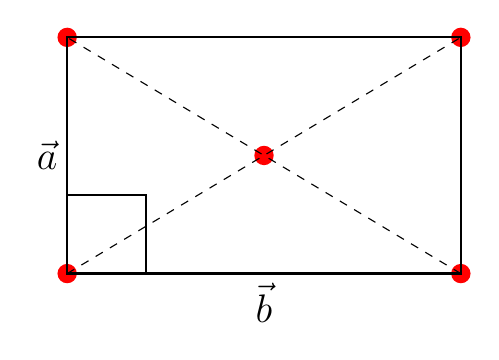
\begin{tikzpicture}
        \def\a{5}  % length of side a
        \def\b{3}  % length of side b
    
        % Calculate the coordinates of the points
        \coordinate (A) at (0, 0);
        \coordinate (B) at (\a, 0);
        \coordinate (C) at (\a, \b);
        \coordinate (D) at (0, \b);
    
        % Creates nodes at vertices
        \fill[red]  (A) circle(3.5pt) (B) circle(3.5pt) (C) circle(3.5pt) (D) circle(3.5pt);
        % Creates nodes at centers
        \fill[red] ($(A)!0.5!(C)$) circle(3.5pt);
    
        % Draw the rectangular unit cell
        \draw[thick] (A) -- (B) -- (C) -- (D) -- cycle;
    
        % Draw lines
        \draw[dashed] (A) -- (C);
        \draw[dashed] (B) -- (D);
    
        % Draw right angle
        \draw[thick] (0,1) -- (1,1) -- (1,0);
            
        %Draw lattice parameters
        \node[left] at ($(A)!0.5!(D)$) {\Large $\vec{a}$};
        \node[below] at ($(A)!0.5!(B)$) {\Large $\vec{b}$};
                
      \end{tikzpicture}}
    
      \vspace{0.5ex}
    
      {\footnotesize\textbf{(d)} Rhombic Cell}
    
      \column{0.3\textwidth}
    
      \resizebox{0.9\columnwidth}{!}{%
      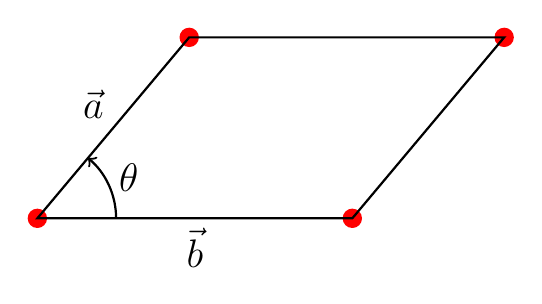
\begin{tikzpicture}
        % Define the lengths of the sides and the angle
        \def\a{4}  % length of side a
        \def\b{3}  % length of side b
        \def\angle{50}  % angle between sides a and b
    
        % Calculate the coordinates of the points
        \coordinate (A) at (0, 0);
        \coordinate (B) at (\a, 0);
        \coordinate (C) at ({\a + \b*cos(\angle)}, {\b * sin(\angle)});
        \coordinate (D) at ({\b * cos(\angle)}, {\b * sin(\angle)});
         
        % Creates nodes at vertices
        \fill[red]  (A) circle(3.5pt) (B) circle(3.5pt) (C) circle(3.5pt) (D) circle(3.5pt);
    
        % Draw the oblique unit cell
        \draw[thick] (A) -- (B) -- (C) -- (D) -- cycle;
    
        %Draw lattice parameters
        \node[anchor={-\angle}] at ($(A)!0.5!(D)$) {\Large $\vec{a}$};
        \node[below] at ($(A)!0.5!(B)$) {\Large $\vec{b}$};
        
        % Optional: add angle markers
        \draw[thick, ->] (A) ++(1,0) arc[start angle=0, end angle=\angle, radius=1] node[midway, anchor={150+\angle}] {\Large $\theta$};
      \end{tikzpicture}}
    
      \vspace{0.5ex}
    
      {\footnotesize\textbf{(e)} Oblique Cell}
    \end{columns}
  % \caption{All five two‐dimensional Bravais unit cells.}
  % \label{fig:bravais-cells}
% \end{figure}

\end{document}